\input{preamble.tex}
\usepackage[a4paper,top=2cm,bottom=2cm,left=2cm,right=2cm]{geometry}
% dove sono le immagini'
\graphicspath{ {./figures/} }

% ACRONIMI
% \newacronym{label}{acronimo}{acronimo esteso}
\newacronym{sts}{STS}{Space Transportation System}
\newacronym{iss}{ISS}{International Space Station}
\newacronym{nasa}{NASA}{National Aeronautics and Space Administration}
\newacronym{ssme}{SSME}{Space Shuttle Main Engine}
\newacronym{srb}{SRB}{Solid Rocket Boosters}
\newacronym{lh2}{$LH_2$}{liquid hydrogen}
\newacronym{lox}{$LO_2$}{liquid oxygen}
\newacronym{lch4}{$LCH_4$}{liquid methane}
\newacronym{lptp}{LPTP}{low pressure turbopump}
\newacronym{hptp}{HPTP}{high pressure turbopump}
\newacronym{et}{ET}{external tank}
\title{ \textbf{Aerospace propulsion final report
\\ Space Shuttle Main Engine: fuel and tank analysis}}
\begin{document}
    \pagenumbering{Roman}
    \maketitle
    \newpage
    \textbf{Abstract}
     
     This project focuses on the redesign of the Space Shuttle Main Engine (SSME), aiming to analyze and optimize the engine's performance first using its original propellant—liquid oxygen (LOX) and liquid hydrogen (LH2)—and subsequently with liquid methane (LCH4) replacing hydrogen. The sizing process was driven by key parameters of the thermodynamic cycle, especially system operating pressures, and included a detailed assessment of the main components, such as the combustion chamber, nozzles, turbopumps, and the external tank.

   The combustion chamber pressure for the methane redesign was estimated based on the Raptor engine developed by SpaceX, which also utilizes liquid methane with liquid oxygen. This estimation allowed for a realistic and practical approach to the redesign process. Importantly, the project emphasizes not just the engine's performance but also the critical aspect of component sizing, particularly in adapting the external tank to accommodate the different oxidizer-to-fuel (O/F) ratios—6.032 for LH2 and 3 for methane.

   In the initial phase, a comprehensive review of the engine's performance using the original propellant was conducted, focusing on combustion chamber pressure and specific impulse (ISP) to establish a baseline. The subsequent redesign phase, incorporating liquid methane, involved adapting key components, including nozzle geometry, expansion ratio, and turbopump characteristics, to maintain optimal efficiency and performance.

   The project demonstrates that liquid methane is a viable alternative, offering benefits in propellant density, chemical stability, and thermal management. However, the primary focus was on the precise sizing of components, particularly ensuring the external tank's capacity and configuration align with the new O/F ratio, while maintaining high combustion chamber pressures to optimize the engine's overall efficiency.
   \newpage
    \tableofcontents
    \newpage
    \printglossary[type=\acronymtype]
    \newpage
    \pagenumbering{arabic}
% --- SCRIVERE QUI ---
    \section{Introduction} \label{intro}
 % Space exploration represents one of the most fascinating and complex frontiers of contemporary science and technology. 
%	At the heart of this field is the \acrfull{sts}, commonly known as the Space Shuttle launch system, which played a fundamental role in the development of human capabilities to explore and utilize space.
	Operated by \acrshort{nasa} from 1981 to 2011, the Space Shuttle was the first reusable space transportation system, an innovative orbital vehicle that combined the characteristics of a rocket and an airplane.
The Space Shuttle program enabled numerous scientific and technical missions, including the launch of satellites, the construction, maintenance of the \acrfull{iss} and a variety of scientific experiments in orbit.
%This vehicle allowed astronauts and payloads to be transported into space and returned to Earth, marking a turning point in the history of astronautics.

The launch system consists of three RS-25 (\acrshort{ssme}) and two additional \acrfull{srb}. The \acrfull{ssme} was one of the most advanced and crucial technological elements of the \acrshort{sts}. The \acrshort{ssme}s were the primary rocket engines, propelled by \acrfull{lh2} and \acrfull{lox}, providing the necessary thrust for the Shuttle's liftoff and initial ascent to low Earth orbit. These engines were known for their efficiency and reliability, being able to operate under extreme conditions and be reused for multiple launches.

    %The Space shuttle propulsion system consists of three space shuttle main engines (SSME) which draw liquid oxigen ($ LO_2 $) and liquid hydrogen ($ LH_2 $) from the external tank (ET).On the sides of the ET two solid rocket boosters are attached.To control the attitude of the orbiter, once it has reached space, two orbital manouvering system (OMS) engines and 44 reaction control systems (RCS) thrusters are used.The following is an analysis of the SSME's thermodynamic cycle and how the propulsive properties change when another fuel is used instead of $ LH_2 $. 

The purpose of this report is to initially size the real \acrfull{ssme} and then, based on the total impulse and burning time of this engine, to resize the engine while changing the fuel from \acrlong{lh2} to \acrfull{lch4}. 
This analysis anticipates a simplification of the system components and a reduction in the mass of the \acrfull{et} given that methane has a much higher density than hydrogen. 
%Additionally, the storage temperature of methane is very similar to that of oxygen, which could help avoid issues related to thermal exchange between the fuel and oxidizer tanks.
The path followed in this report involved taking upstream and downstream pressures of each component, the inlet temperatures to the various components, and the mass flow rates of the fuel and oxidizer.
Using these parameters, the turbopumps, injectors, combustion chamber, nozzle, and \acrlong{et} were appropriately sized through MATLAB. For the engine's performance analysis, NASA's CEA software was utilized.
Subsequently, by observing these performances and using the burning time, O/F ratio, total engine impulse, and combustion chamber pressure as starting points, the engine was resized for the new fuel (\acrshort{lch4}) by working backward from these parameters.

(immagine del motore e del sistema di lancio dello shuttle) immagini da mettere una a destra e una a sinistra con il testo intorno

%\begin{figure}
%	\centering
 %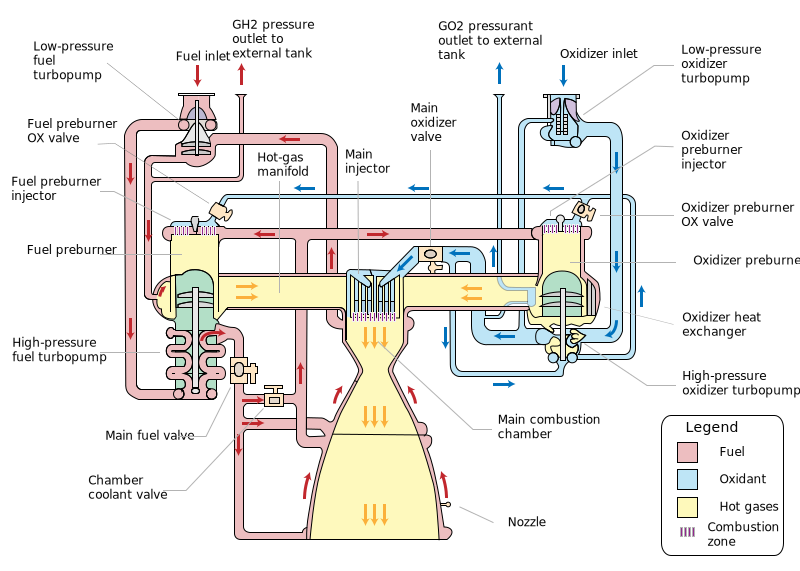
\includegraphics[width=.50\textwidth]{ssme_ciclo}
%	\caption{A functional diagram showing the flow of propellant through an RS-25 engine.}
%	\label{fig:ssme_cycle}
%\end{figure}

\subsection{Introduction to the staged combustion cycle}
The Stage Combustion Cycle used in the Space Shuttle Main Engine (SSME) is a highly efficient and intricate system specifically designed for maximum performance.
In the SSME, this cycle involves the partial combustion of both liquid hydrogen (fuel) and liquid oxygen (oxidizer) in separate preburners. 
The preburners produce hot, high-pressure, fuel-rich gases that drive the engine's turbopumps, which in turn feed the remaining propellants into the main combustion chamber at extremely high pressures.
What sets the SSME apart is its use of a closed-cycle stage combustion process, where all the exhaust gases from the preburners are directed into the main combustion chamber, ensuring that no energy is wasted.
This results in very high efficiency, with the SSME achieving one of the highest specific impulses of any rocket engine.
The high pressures and temperatures involved in this cycle make it extremely complex, but they also enable the SSME to deliver the power needed for the Space Shuttle's demanding missions.
\begin{figure}[H]
	\centering
 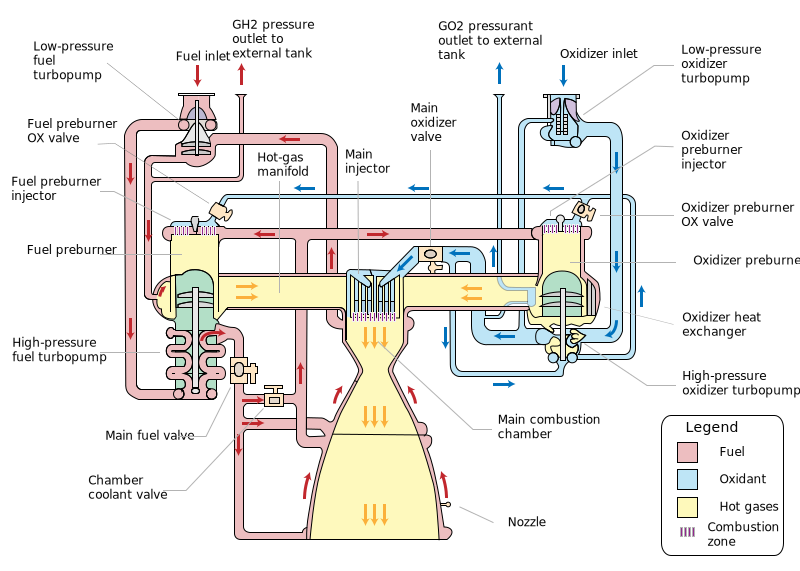
\includegraphics[width=.50\textwidth]{ssme_ciclo}
	\caption{A functional diagram showing the flow of propellant through an RS-25 engine.}
	\label{fig:ssme_cycle}
\end{figure}

\subsection{Introduction to Liquid Hydrogen and Liquid Methane}
Liquid hydrogen is renowned for its exceptionally high specific impulse, which means it can generate more thrust per unit mass compared to other propellants.
This makes it ideal for missions where maximizing fuel efficiency is crucial. 
Hydrogen is particularly well-suited for use in advanced propulsion cycles like the Stage Combustion Cycle employed by the SSME, where the goal is to extract the maximum amount of energy from the propellant.
However, liquid hydrogen has a very low density (about 70.85 kg/m³ at 20.27 K), necessitating larger and heavier tanks to store the same amount of energy as denser fuels.
This increases the overall mass of the vehicle and complicates volume management.
Furthermore, hydrogen must be stored at extremely low temperatures (around 20.27 K), which is significantly lower than the boiling point of liquid oxygen (90 K).
This substantial temperature difference presents considerable challenges in tank design and thermal management, increasing the risk of unwanted heat transfer between the fuel and oxidizer tanks.
Additionally, because hydrogen molecules are very small, they can easily escape through micro-cracks or porous materials, increasing the likelihood of leaks.

Liquid methane, in contrast, has a much higher density (about 422.62 kg/m³ at 100 K), allowing for a reduction in the volume of the tanks required to store the fuel, which in turn reduces the overall mass and size of the tanks.
This can lead to improvements in vehicle efficiency.
Methane can be stored at a temperature close to that of liquid oxygen (100 K), which minimizes the challenges related to thermal management and reduces the risk of heat exchange issues between the fuel and oxidizer tanks.
Moreover, methane is easier to handle than hydrogen, as it does not require storage at extremely low temperatures and does not pose the same level of risk for leaks due to its larger molecular size.
However, methane has a lower specific impulse compared to hydrogen, meaning it is less efficient at converting fuel mass into thrust.
This results in a reduction in overall engine efficiency and performance. Additionally, the combustion of methane can lead to the production of soot, which can complicate residue management and engine maintenance.

\section{Problem analysis}
The starting point for the analysis involves collecting data on pressures and temperatures from official documents found on the web for the staged combustion cycle of the RS-25, both upstream and downstream of the original engine components. 
This data is then used to size these components and calculate the engine's performance. 
In the second part of the analysis, the process is reversed: starting from the desired performance, the engine is sized for the new fuel. 
The sizing focuses on the turbopumps, preburners (injectors), combustion chamber, nozzle, and external tank, while simplified assumptions are made for other parts of the engine, such as engine cooling, heat exchangers, and feed lines.

\subsection{Turbopumps design}
The Space Shuttle Main Engine (SSME) turbopump system consists of four main turbopumps, each playing a critical role in the engine's operation. These include the High-Pressure Oxygen Turbopump (HPOTP) and the Low-Pressure Oxygen Turbopump (LPOTP), as well as the High-Pressure Fuel Turbopump (HPFTP) and the Low-Pressure Fuel Turbopump (LPFTP). Together, these turbopumps increase the propellant pressure to extremely high levels, necessary for injection into the combustion chamber

When designing a turbopump for space propulsion, several key parameters need to be calculated to ensure the pump operates efficiently and meets the specified requirements. Given the known fluid characteristics and operational demands, the following equations are used to determine the design elements of the pump.

\subsubsection{Pump key design parameters}
\begin{itemize}
    
 \item\textbf{Pressure Differential and Head of the pump}

The pressure differential (\(\Delta P\)) across the pump is given by:
\[
\Delta P = P_{\text{out}} - P_{\text{in}}
\]

The head (\(H\)) of the pump, which represents the energy imparted to the fluid, is calculated as:
\[
H = \frac{\Delta P}{g \cdot \rho}
\]

\item\textbf{Number of Stages}

The number of stages (\(N_s\)) required for the pump is determined based on the maximum theoretical pressure differential per stage (\(\Delta P_{\text{ps}}\)) and the overall pressure differential.
This theoretical pressure differential per stage is set with 16 Mpa for the liquid hydogen while 47 Mpa for other cryogenic fluids, according to the design guidelines of the book "Space Propulsion Analysis and Design"(DA INSERIRE BIBLIOGRAFIA).
\[
N_s = \left\lceil \frac{\Delta P}{\Delta P_{\text{ps}}} \right\rceil
\]
where \(\lceil \cdot \rceil\) denotes the ceiling function.

\item\textbf{Rotational Speed of the shaft}

The rotational speed (\(V_r\)) of the pump and turbine shaft is calculated using the stage specific speed (\(V_s\)) and the pump head divided by the number of stages. For a pump without a booster:
\[
V_r = \frac{V_s \cdot \left(\frac{H}{N_s}\right)^{0.75}}{\sqrt{Q}}
\]
where \(Q\) is the volumetric flow rate:
\[
Q = \frac{\dot{m}}{\rho}
\]
The stage-specific speed is set based on extensive testing to ensure that the results closely match the data of the actual turbopumps.

The rotational speed in revolutions per minute (rpm) is:
\[
V = \frac{30 \cdot V_r}{\pi}
\]

\item\textbf{Outlet Temperature}

The outlet temperature (\(T_{\text{out}}\)) of the fluid is determined by adding the temperature change to the inlet temperature (\(T_{\text{in}}\)). The temperature change (\(\Delta T\)) is calculated using the enthalpic change and specific heat capacity (\(c_p\)):
\[
\Delta T = \frac{\Delta H}{c_p}
\]
where the enthalpic change (\(\Delta H\)) is:
\[
\Delta H = \frac{P_{\text{req}}}{\dot{m}}
\]
and \(P_{\text{req}}\) is the power required to drive the pump:
\[
P_{\text{req}} = \frac{g \cdot \dot{m} \cdot H}{\eta_{\text{pump}}}
\]
with \(\eta_{\text{pump}}\) being the efficiency of the pump.

Thus:
\[
T_{\text{out}} = T_{\text{in}} + \Delta T
\]

\item\textbf{Power Required}

The power required (\(P_{\text{req}}\)) to drive the pump is given by:
\[
P_{\text{req}} = \frac{g \cdot \dot{m} \cdot H}{\eta_{\text{pump}}}
\]

\end{itemize}

During the compression process of the HPFTP, it was observed that the fluid reached supercritical conditions. This transition to supercritical conditions led to significant discrepancies between the theoretical results and the actual data. Supercritical fluids exhibit altered physical properties, which complicates the accuracy of a comprehensive pump analysis.

To address this issue and improve the precision of the results, a different approach was adopted only for this pump. Instead of analyzing the pump as a single unit, it was divided into its three distinct stages. This subdivision allowed for a detailed analysis of each stage individually.

By examining each stage separately, it was possible to have better control over the physical characteristics of the fluid throughout the various phases of the compression process. This approach facilitated the adjustment of design conditions to reflect the specific operational realities of each stage of the pump. Consequently, the results obtained were much closer to the actual experimental data, enhancing the reliability and accuracy of the pump design.

\subsubsection{Turbines key design parameters}

\begin{itemize}
    \item \textbf{Pressure Ratio}
    
    The pressure ratio is given by:
    \[
    \beta = \frac{p_{\text{in}}}{p_{\text{out}}}
    \]

    \item \textbf{Power Required}
    
    The power required from the turbine is set equal to that of the respective pump:
    \[
    P_{\text{req}} = \frac{P_{\text{tp}}}{\eta_{\text{mech}}}
    \]
    where \( \eta_{\text{mech}} = 0.81 \) is the total mechanical efficiency, calculated as \( \eta_{\text{pump}} \times \eta_{\text{turbine}} \) with both efficiencies assumed to be \(0.9\).

    \item \textbf{Outlet Temperature} 
    
    The outlet temperature is calculated as:
    \[
    T_{\text{out}} = T_{\text{in}} - \left(\eta_{\text{turb}} \times \left(T_{\text{in}} - T_{\text{out,id}}\right)\right)
    \]
    where \(T_{\text{out,id}}\) is the ideal outlet temperature determined by:
    \[
    T_{\text{out,id}} = T_{\text{in}} \left(\frac{1}{\beta}\right)^{\frac{\gamma - 1}{\gamma}}
    \]

    \item \textbf{Isoentropic Spouting Velocity} 
    
    The isoentropic spouting velocity, representing the velocity the turbine gas flow would have if expanded isoentropically from the turbine inlet to the outlet pressure, is calculated as:
    \[
    C_0 = \sqrt{2 \cdot c_p \cdot T_{\text{in}} \left(1 - \left(\frac{1}{\beta}\right)^{\frac{\gamma - 1}{\gamma}}\right)}
    \]

\item\textbf{Number of stage}

In this case the number of the turbines stages is taken by the official documents that describe the turbines.
\end{itemize}
%da inserire tabella con i dati
\subsection{Preburners and injectors design}

The Space Shuttle Main Engine (SSME) employs a sophisticated preburner system designed to efficiently initiate and sustain the combustion process in its main combustion chamber. The SSME features two preburners: one for the liquid hydrogen (LH2) and one for the liquid oxygen (LOX).

The preburners are essentially small combustion chambers where a portion of the propellant is burned to produce high-pressure, high-temperature gases. These gases are then used to drive the turbopumps that supply the main combustion chamber with propellants.
This staged combustion results in a highly efficient process where the majority of the propellant is burned in the main combustion chamber.

By utilizing this staged combustion technique, the SSME achieves high performance and efficiency, which is critical for the demanding requirements of space shuttle launches.

\subsubsection{Preburners combustion: Nasa CEA analysis}
For the combustion process within the preburners, the NASA's CEA software was utilized to model and analyze the combustion characteristics under fixed enthalpy and pressure conditions. The software was configured to solve combustion problems by specifying the oxidizer-to-fuel (O/F) ratios, which varied depending on whether methane or hydrogen was used as the fuel. The analysis incorporated the chemical species and their respective temperatures, which were determined from previous pumps analyses.

 The software provided detailed information on the combustion products and their thermophysical properties. 
 This analysis is crucial because the exhaust gases, after passing through the High-Pressure Turbopumps' turbines (HPTP), enter the combustion chamber.
 Understanding the properties of these gases ensures that the combustion chamber operates efficiently and effectively under the conditions dictated by the preburner’s output.

\subsubsection{Injector design}
The selected injector type is a coaxial injector, where the oxidizer flows through a central core and the fuel flows in an annular ring surrounding the core. This design is considered highly efficient for cryogenic fluids. The coaxial configuration ensures optimal mixing and combustion efficiency by leveraging the high efficiency of the coaxial injector design for cryogenic propellants.

Given the mass flow rates of liquid oxygen (LOX) and fuel, their densities, and the pressure differentials across the injectors, this analysis aims to determine the number and size of injectors needed to achieve the desired mass flow rates for both propellants.

Initially, the areas for LOX and fuel injectors are set to \(5 \times 10^{-6}\) m² and \(1 \times 10^{-5}\) m², respectively. These values serve as starting points for the calculations. A convergence tolerance of \(1 \times 10^{-10}\) and a maximum of 1000 iterations are defined to ensure accurate results.

The process involves iteratively refining the injector areas until convergence is achieved or the maximum number of iterations is reached.


In each iteration, the exit velocities of LOX and fuel are calculated using the pressure differential and densities. The velocity is determined by the formula:
\[
V = \sqrt{\frac{2 \cdot \Delta P}{\rho}}
\]
The mass flow rate through each injector is then computed using these velocities and the current injector areas.

Based on the mass flow rates of LOX and fuel, the number of injectors required is calculated. This is done by dividing the total mass flow rate by the mass flow rate of a single injector and then taking the ceiling of the maximum value to ensure an adequate number of injectors.

New injector areas are calculated based on the desired mass flow rates and the number of injectors. The new area for each injector is given by:
\[
\text{New Area} = \frac{\dot{m}}{(\text{Number of Injectors} \times \rho \cdot V)}
\]

The loop terminates when the change in injector area is smaller than the specified tolerance for both LOX and fuel, indicating that convergence has been achieved.

Upon convergence, additional parameters are calculated:
\begin{itemize}
    \item \textbf{Diameter of LOX Injector}: Determined using the formula for the area of a circle: \[
D_{\text{LOX}} = \sqrt{\frac{4 \cdot A_{\text{LOX}}}{\pi}}
\]
    \item \textbf{Thickness of Fuel Injector}: Calculated as the difference between the new fuel area and the LOX injector diameter: \[
\text{Spessore}_{\text{fuel}} = \sqrt{\frac{A_f + A_{\text{LOX}}}{\pi}} - \frac{D_{\text{LOX}}}{2}
\]
\end{itemize}

\subsection{Combustion chamber design}
\subsection{Performances calculation}
The performance analysis of the engine was conducted for both hydrogen and methane fuels using NASA's Chemical Equilibrium with Applications (CEA) software. 
The problem was set up as a rocket combustion analysis, utilizing known parameters such as the combustion chamber pressures and the expansion ratio. 
For the combustion chamber pressures, the values for hydrogen were taken from official documentation of classic engine (19.7 Mpa), while for methane, estimates were derived based on observations from the RS-25 engine and the SpaceX Raptor engine (21.5 Mpa) , the latter being a methalox engine.

Regarding the expansion ratio, it was set to the original value used for the RS-25 engine, which is \(\varepsilon = 69\), for both hydrogen and methane cases.
This consistent expansion ratio allows for a comparative analysis of engine performance under similar operational conditions. 
The CEA software provided insights into the thermodynamic properties and performance metrics, such as specific impulse and thrust, which are essential for evaluating the efficiency and effectiveness of the propulsion system.

In the combustion analysis performed using NASA's CEA software, the chemical species were selected to accurately represent the real combustion environment. For the fuel component, the products of combustion from the preburners were used, reflecting the actual gases that participate in the main combustion process. These preburner combustion products were specifically chosen to capture the true chemical composition and thermodynamic properties of the gases involved. As for the oxidizer, liquid oxygen was used, which is a standard choice for such analyses due to its role as the primary oxidizing agent in rocket propulsion systems.

(tabella con le specie chimiche)

In the combustion analysis for both hydrogen and methane, the oxidizer-to-fuel (O/F) ratios were chosen based on specific references to ensure realistic and accurate performance evaluations. For hydrogen, an O/F ratio of 6.032 was used, which corresponds to the value specified for the original engine design. This ratio reflects the optimal conditions for hydrogen combustion in the given engine configuration. In contrast, for the methane case, an O/F ratio of 3 was utilized, as documented in the literature (Sutton). This ratio is representative of the typical conditions used in methane-based propulsion systems and provides a comparative basis for evaluating the performance of methane versus hydrogen as propellants. These O/F ratios are crucial for determining the combustion efficiency and overall engine performance in the analysis.
This setup ensures that the analysis accurately represents the combustion conditions and provides relevant performance metrics for both hydrogen and methane fuels.
The outputs from the NASA CEA software that were utilized in the analysis include several key parameters: specific impulse, characteristic velocity, speed of sound at the nozzle exit, and the pressures and temperatures at the combustion chamber, throat, and exit sections. From the exit pressure, it is possible to infer the altitude at which the engine operates at optimal expansion. Additionally, important data regarding the combustion products were obtained, such as their density, specific heat capacity (\(c_p\)), specific heat ratio (\(\gamma\)) and moleculr mass of the exhaust gases (\(M_m\)). These outputs provide crucial information for understanding the engine's performance and the behavior of the exhaust gases under various conditions.

Using the data obtained from the NASA CEA software, we can calculate key performance metrics for the engine. The exhaust velocity (\(V_e\)) at the nozzle exit is calculated using the following equation:

\[
V_{e} = \sqrt{\left(\frac{2 \gamma}{\gamma - 1}\right) R T_{c} \left(1 - \left(\frac{p_{e}}{p_{c}}\right)^{\frac{\gamma - 1}{\gamma}}\right)}
\]

where \( \gamma \) is the specific heat ratio of the exhaust gases, \( R\) is the specific gas constant, \( T_{c} \) is the combustion chamber temperature, \( p_{e} \) is the exit pressure, and \( p_{c} \) is the combustion chamber pressure.

The thrust (\( T \)) produced by the engine is given by:

\[
 T = \dot{m}_{p} \cdot V_{e}
\]

where \( \dot{m}_{p} \) is the mass flow rate of the propellant.

Finally, the total impulse (\( I_{\text{tot}} \)) of the engine over the entire burn duration is calculated as:

\[
I_{\text{tot}} = T \cdot \text{burning\_time}
\]

It's important to note that the burning time used in this calculation is 480 seconds, corresponding to the original engine's burn duration.

The total impulse and the burning time are the starting point for the design of the engine using the methane.

\subsection{External Tank design}

\subsection{Nozzle Design and Profile Generation}
This section covers the design and dimensioning of the converging-diverging nozzle of the SSME, including a 2D and 3D profile generation
\subsubsection{Nozzle sizing}
The sizing process involves the use of the nozzle's performance parameters:


\begin{itemize}
    \item Specific impulse (\(I_{sp}\)) at sea level;
    \item Burn time: \(480 \, \text{s}\);
    \item Chamber pressure (\(p_c\));
    \item Exit pressure (\(p_e\));
    \item Chamber Temperature (\(T_c\)) ;
    \item Specific Velocity (\(c^*\)) ;

\end{itemize}
Given those data, the following calculations are performed to size the nozzle:
        \begin{itemize}
        \item\textbf {Throat area (\(A_t\)):}
        \[
A_t = \frac{\dot{m}_p}{c^* \cdot p_c}
\]
            \item\textbf {Throat Diameter (\(D_t\)):} 
            
            is calculated from the throat area (\(A_t\)):
            \[
            D_t = \sqrt{\frac{4 A_t}{\pi}}
            \]
            
            \item \textbf{Exit Diameter (\(D_e\)):}
            
            is obtained using the expansion ratio (\(\epsilon\)) and throat diameter:
            \[
            A_e = \varepsilon \cdot A_t
            \]
            \[
            D_e = \sqrt{\frac{4 A_e}{\pi}}
            \]
            
            \item \textbf{Combustion Chamber Volume (\(V_c\)) and Length (\(L_c\)):}
            \[
            V_c = L^* \cdot A_t
            \]
            \[
            L_c = \frac{V_c}{A_c}
            \]
            where \(L^*\) is the specific length and is set to be 1.14 m for both the classic RS-25 nozzle and the modified engine's one.
    \end{itemize}
              The length of the diverging and converging (combustion chamber) sections are scaled by a Bell factor \(K\). In this case, \(K = 0.75\). The adjusted lengths are:
    \[
    L_c = L_c \times K
    \]
    \[
    L_d = L_d \times K
    \]

\subsubsection{Nozzle Profile Generation}

The nozzle profile is generated using a MATLAB function that produces a converging-diverging nozzle shape. The profile is divided into converging and diverging sections with the following characteristics:

\begin{itemize}
    \item \textbf{Converging Section:} The radius decreases linearly from the combustion chamber radius (\(R_c\)) to the throat radius (\(R_g\)). The radius as a function of the distance \(x\) along the converging section is given by:
    \[
    y_{\text{conv}} = R_c - \left( R_c - R_g \right) \frac{x}{L_c}
    \]

    \item \textbf{Diverging Section:} The diverging section is modeled as a parabolic curve. The parabola's coefficients are calculated to ensure the profile transitions smoothly from the throat to the exit. The parabolic equation is:
    \[
    y_{\text{div}} = a x^2 + b x + c
    \]
    where \(a\), \(b\), and \(c\) are determined by solving a system of equations that ensures the correct shape of the profile and the desired angle of divergence (\(\alpha_{\text{div}}\)).


To determine the convergent-divergent nozzle profile, the coefficients \(a\), \(b\), and \(c\) of the divergent parabola were calculated to satisfy the conditions at the throat and exit sections, including the slope at the throat determined by the divergence angle \(\alpha_{div}\). The system of equations is:

\[
a R_g^2 + b R_g + c = 0
\]

\[
a R_e^2 + b R_e + c = L_d
\]

\[
2a R_g + b = \frac{1}{\tan(\alpha_{div})}
\]

Where:
\begin{itemize}
    \item \(R_g\) is the radius at the throat section,
    \item \(R_e\) is the radius at the exit section,
    \item \(L_d\) is the length of the divergent section,
    \item \(\alpha_{div}\) is the divergence angle.
\end{itemize}


Once the 2D profile of the nozzle is determined, it is revolved around the central axis to create a 3D mesh. The points along the profile are rotated through 360 degrees to form the surface of the nozzle.

Finally, the generated 3D nozzle profile is visualized using a \texttt{patch} function that displays the surface with specified color and transparency settings. This provides an intuitive understanding of the nozzle's geometry and ensures that the design meets the required specifications.

This approach offers a detailed and accurate representation of the nozzle profile, which is critical for ensuring the optimal performance of the rocket engine. The final 3D model can also be exported as an STL file for further analysis or manufacturing.

\end{itemize}

\subsection{Modified RS-25 deign path}
The design of the modified RS-25 started with the idea of replying the total impulse of the original engine. The other starting points were the burning time of the original engine, the O/F of 3 and the performances calculated with the analysis carried out with NASA Cea. Other hypotesis  were made to complete the analysis:
\begin{itemize}
    \item\textbf{Temperature and pressure in the Tank:}

    those two data were taken looking up to the Raptor engine by SpaceX and were set to be 100 K and 0.2 Mpa ;

    \item\textbf{Pressures along the fuel line:} 
    the pressures along the tubes of the fuel line were taken mostly equal to the cas of LH2 engine so to simplify the analysis of the modified engine ;

    \item\textbf{Turbopumps characteristic:}
    The pressure rise and drop in the turbopumps were set to be similar to the LH2 turbopumps, same as the number of stages in the turbines. Also the type of pumps were not changed. 
    \item \textbf{Oxidizer line:}
    the oxidizer line is mantained the same as the one of the original RS-25, that because after the calculations of the masses flow nedeed to reach the required specific impulse it was noticed that it is almost equal 
    \item\textbf{Nozzle expansion ratio}
\end{itemize}
\section{Discussion of results}
\subsection{Classic RS-25}
\subsection{Modified RS-25}
\section{Conclusions}

 \end{document}
%%% TeX-master: t